
\section{三维坐标轴配置}
\label{sec:3d:axis:config}

{
\tikzset{external/figure name/.add={}{threedimaxis_}}

本节描述用于配置三维图形外观的键。其中有些键在二维绘图的特殊情形下同样适用，它们也会在本手册相应章节中讨论。


\subsection{视图配置}

\begin{pgfplotskey}{view=\marg{azimuth}\marg{elevation} (initially \{25\}\{30\})}
\index{3d view!Assign rotation angles}%
\index{View!Assign rotation angles}%
    修改三维坐标轴的两个视角方位角。方位角（第一个参数）是绕 $z$ 轴旋转的水平角。对于三维绘图，$z$ 轴始终指向顶部。仰角（第二个参数）是绕（已旋转的）$x$ 轴的垂直旋转角。正的仰角值表示从上方俯视，负值表示从下方仰视。所有角度均以度为单位（但参见 |trig format|）。
    %
\pgfplotsexpensiveexample
\begin{codeexample}[]
\begin{tikzpicture}
\begin{axis}[
    view={0}{0},
    xlabel=$x$,
    zlabel=$z$,
    title=View along the positive $y$-axis,
]
    \addplot3 [surf] {x};
\end{axis}
\end{tikzpicture}
\end{codeexample}

\pgfplotsexpensiveexample
\begin{codeexample}[]
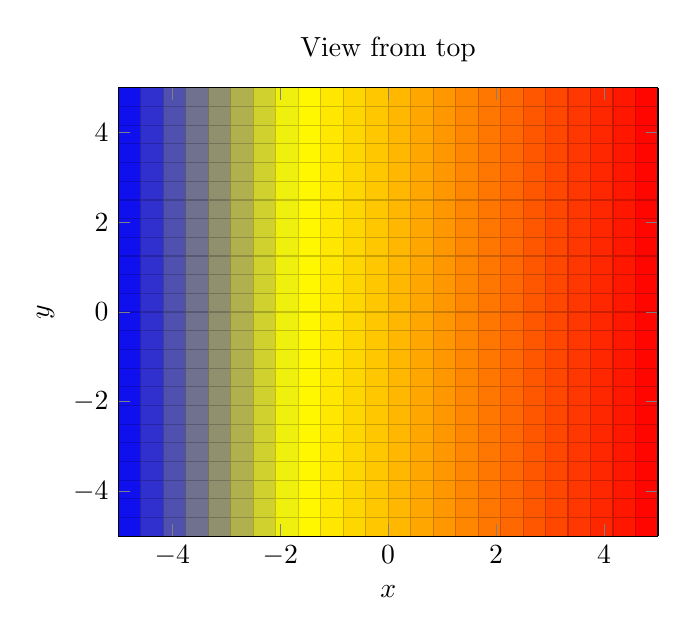
\begin{tikzpicture}
\begin{axis}[
    view={0}{90},
    xlabel=$x$,
    ylabel=$y$,
    title=View from top,
]
    \addplot3 [surf] {x};
\end{axis}
\end{tikzpicture}
\end{codeexample}

\pgfplotsexpensiveexample
\begin{codeexample}[]
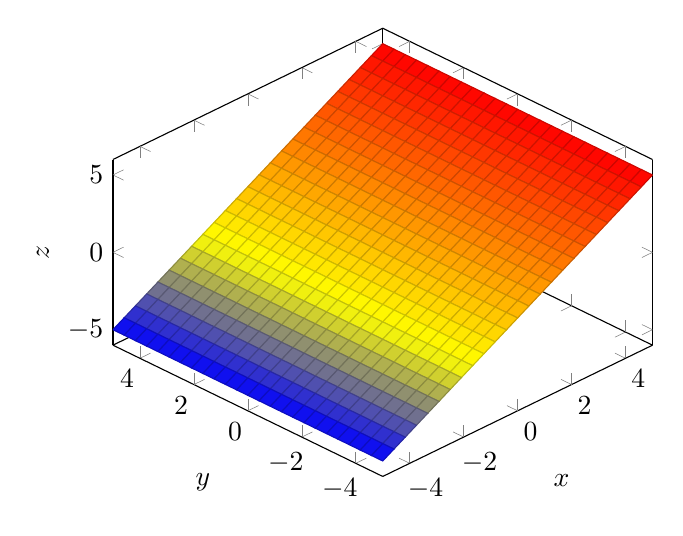
\begin{tikzpicture}
\begin{axis}[
    view={-45}{45},
    xlabel=$x$,
    ylabel=$y$,
    zlabel=$z$,
]
    \addplot3 [surf] {x};
\end{axis}
\end{tikzpicture}
\end{codeexample}

    |view| 的计算方式如下。视图由两次旋转定义：第一次旋转使用 \meta{azimuth} 角绕 $z$ 轴旋转。之后，视图绕 \emph{已旋转的} $x$ 轴旋转 \meta{elevation} 度（更准确地说，是旋转 $-$\meta{elevation} 度）。变换后得到的 $xz$ 平面即为视口，也就是说，视图方向始终是变换后的正 $y$ 轴方向。

    |view| 参数与 Matlab$^\text{\textregistered}$ 的 view 命令的参数兼容，也就是说，你可以在 Matlab 中使用

    |[h,v] = view|

    \noindent 并将得到的参数传入 \PGFPlots{}。\footnote{如果不奏效，请在 \PGFPlots{} 中尝试 \texttt{h} 和 \texttt{-v}。}

    如果你使用 |gnuplot|，可以按如下方式转换视图参数：|gnuplot| 命令

    |set view v,h|

    \noindent 与 |view={h}{90-v}| \emph{等价}。例如，默认的 |gnuplot| 配置 |set view 60,60| 等价于 \PGFPlots{} 中的 |view={60}{30}|。

    |view|（目前）始终是正交投影，尚不能实现透视投影。不过，你可以显式地为 |x|、|y| 和 |z| 指定投影单位向量，以得到倾斜的三维坐标轴。
\end{pgfplotskey}

\begin{pgfplotskeylist}{view/az=\marg{azimuth},view/h=\marg{azimuth} (initially 25)}
    仅修改方位角视角，也就是绕 $z$ 轴旋转的水平（第一）视角角。
    %
\pgfplotsexpensiveexample
\begin{codeexample}[]
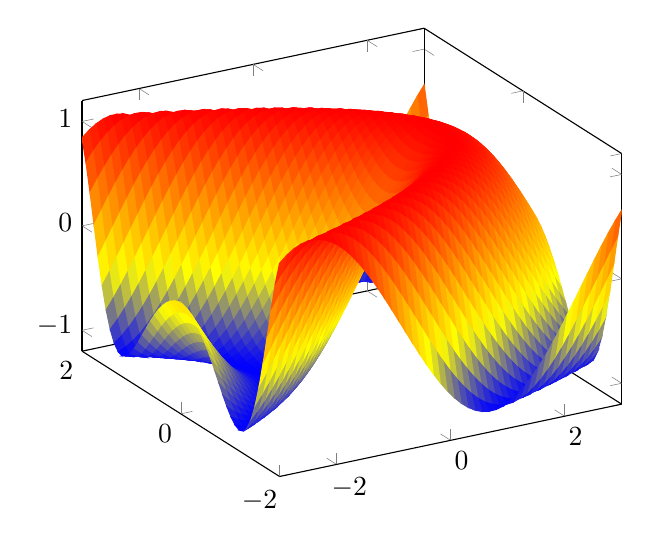
\begin{tikzpicture}
\begin{axis}[view/h=-30]
    \addplot3 [
        surf,
        %shader=interp,
        shader=flat,
        samples=50,
        domain=-3:3,y domain=-2:2,
    ]
        {sin(deg(x+y^2))};
\end{axis}
\end{tikzpicture}
\end{codeexample}

\pgfplotsexpensiveexample
\begin{codeexample}[]
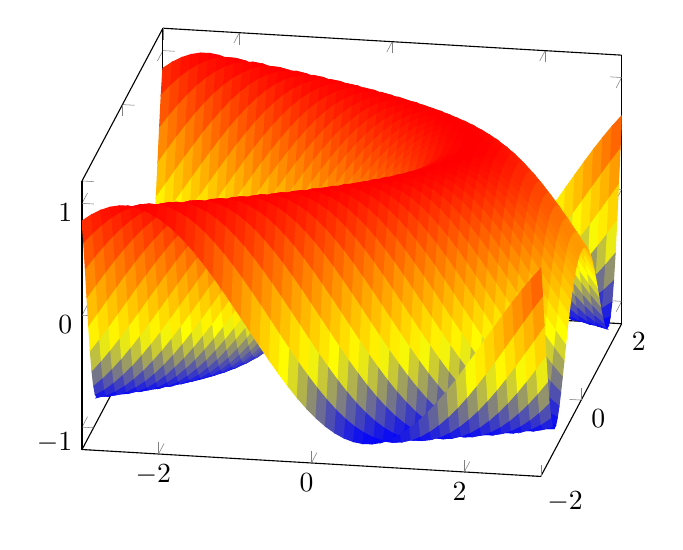
\begin{tikzpicture}
\begin{axis}[view/h=10]
    \addplot3 [
        surf,
        %shader=interp,
        shader=flat,
        samples=50,
        domain=-3:3,y domain=-2:2,
    ]
        {sin(deg(x+y^2))};
\end{axis}
\end{tikzpicture}
\end{codeexample}

\pgfplotsexpensiveexample
\begin{codeexample}[]
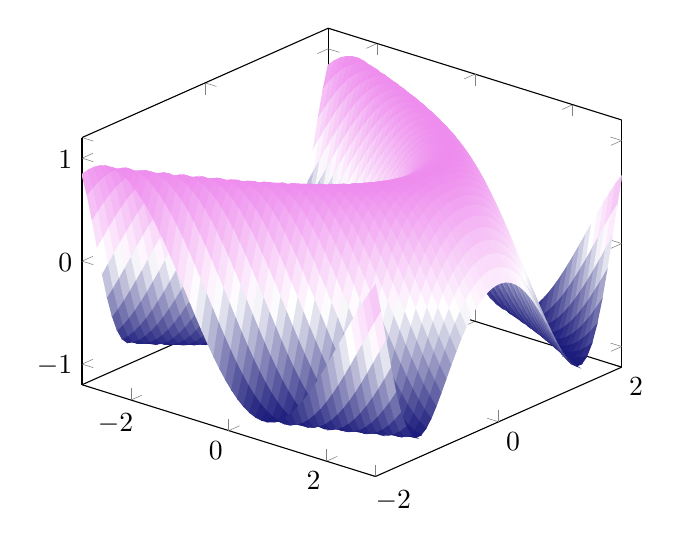
\begin{tikzpicture}
\begin{axis}[view/h=40,colormap/violet]
    \addplot3 [
        surf,
        %shader=interp,
        shader=flat,
        samples=50,
        domain=-3:3,y domain=-2:2,
    ]
        {sin(deg(x+y^2))};
\end{axis}
\end{tikzpicture}
\end{codeexample}

\pgfplotsexpensiveexample
\begin{codeexample}[]
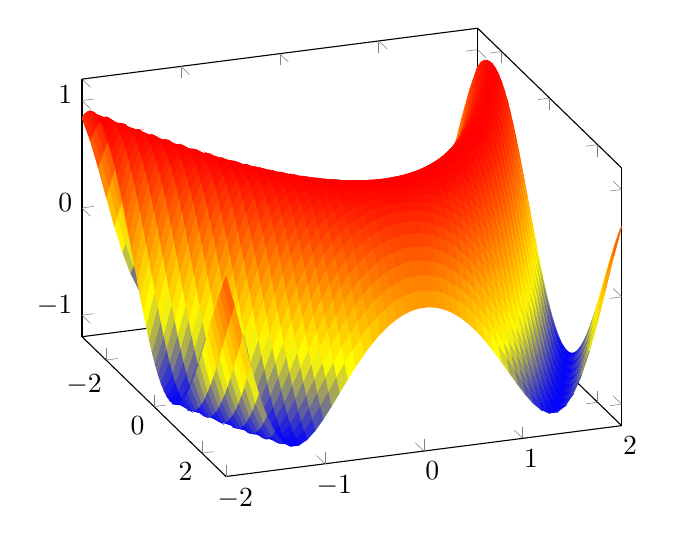
\begin{tikzpicture}
\begin{axis}[view/h=70]
    \addplot3 [
        surf,
        %shader=interp,
        shader=flat,
        samples=50,
        domain=-3:3,y domain=-2:2,
    ]
        {sin(deg(x+y^2))};
\end{axis}
\end{tikzpicture}
\end{codeexample}
\end{pgfplotskeylist}

\begin{pgfplotskeylist}{view/el=\marg{elevation},view/v=\marg{elevation} (initially 30)}
    仅修改垂直仰角，也就是 |view| 的第二个参数。正值表示从上方俯视，负值表示从下方仰视。
\end{pgfplotskeylist}


\subsection{仅用于三维坐标轴的样式}

\begin{stylekey}{/pgfplots/every 3d description}
    此样式允许修改三维坐标轴 \emph{描述} 的外观。自然地，三维坐标轴显示 $x$ 和 $y$ 坐标轴标签的方式与二维坐标轴不同（例如，$y$ 轴标签不会旋转 90 度）。|every 3d description| 样式为三维坐标轴描述安装了必要的显示选项。

    初始值为：
    %
\begin{codeexample}[code only]
\pgfkeys{
    /pgfplots/every 3d description/.style={
        % Only these description styles can be changed here:
        every axis x label/.style={
            at={(ticklabel cs:0.5)},
            anchor=near ticklabel,
        },
        every axis y label/.style={
            at={(ticklabel cs:0.5)},
            anchor=near ticklabel,
        },
        every x tick scale label/.style={
            at={(xticklabel cs:0.95,5pt)},
            anchor=near xticklabel,
            inner sep=0pt,
        },
        every y tick scale label/.style={
            at={(yticklabel cs:0.95,5pt)},
            anchor=near yticklabel,
            inner sep=0pt,
        },
        try min ticks=3,
    },
}
\end{codeexample}

    顾名思义，|every 3d description| 只能用于设置坐标轴标签、刻度标签和标题的样式。它\emph{并非}为重置其他样式而设计，你需要单独为每个坐标轴更改这些选项，或者通过用户自定义样式来更改。此限制的原因是：其他选项可以（而且在很多情况下必须）在坐标轴被处理之前设置。然而，我们究竟拥有二维坐标轴还是三维坐标轴，这一判断必须推迟到处理过程大致完成之后——因此只有一些剩余的键可以被设置。
\end{stylekey}

\begin{stylekey}{/pgfplots/every 3d view \marg{h}\marg{v}}
    一个可用于针对特定视图微调输出的样式。

    此样式会在 |every 3d description| 之后、但在其他与坐标轴描述相关的键被设置之前立即安装（换句话说：它的优先级高于 |every 3d description|，但低于直接提供给坐标轴的键）。

    已经为 |view={0}{90}|（从上方俯视）预配置了一个示例：
    %
\begin{codeexample}[code only]
\pgfplotsset{
    /pgfplots/every 3d view {0}{90}/.style={
        xlabel near ticks,
        ylabel near ticks,
        axis on top=true,
    },
}
\end{codeexample}
\end{stylekey}


\subsection{三维盒的外观}

\begin{pgfplotskey}{plot box ratio=\marg{\meta{x stretch} \meta{y stretch} \meta{z stretch}} (initially 1 1 1)}
    允许自定义三维绘图中三个不同坐标轴之间的纵横比。

    请注意，此键与相关的 |unit vector ratio| 不同：plot box 仅对三维坐标轴有用，而且它通常会扭曲单位向量比。如果你希望单位比相等，请考虑使用 |unit vector ratio|。

    |plot box ratio| 在任何旋转和拉伸填充例程被调用\emph{之前}应用。因此，初始设置\footnote{请注意，你也可以使用语法 \texttt{\{1\}\{1\}\{1\}} 来代替空格分隔。} |1 1 1| 会在应用拉伸填充例程之前，使所有坐标轴长度相等。
    %
\pgfplotsexpensiveexample
\begin{codeexample}[]
\begin{tikzpicture}
\begin{axis}[
    view/h=60,
    plot box ratio=1 1 1,
    colormap={violet}{[1cm] rgb255(0cm)=(25,25,122)
        color(1cm)=(white) rgb255(5cm)=(238,140,238)},
    xlabel=$x$,
    ylabel=$t$,
    zlabel={$p(x,t)$},
    shader=faceted,
    title=Initial \texttt{plot box ratio},
]
    \addplot3 [surf,y domain=0.02:3.5,samples=81]
        {1/(2*sqrt(pi*y)) * exp(0-x^2/y)};
    % the '0' is a workaround for a bug in PGF 2.00
\end{axis}
\end{tikzpicture}
\end{codeexample}

\pgfplotsexpensiveexample
\begin{codeexample}[]
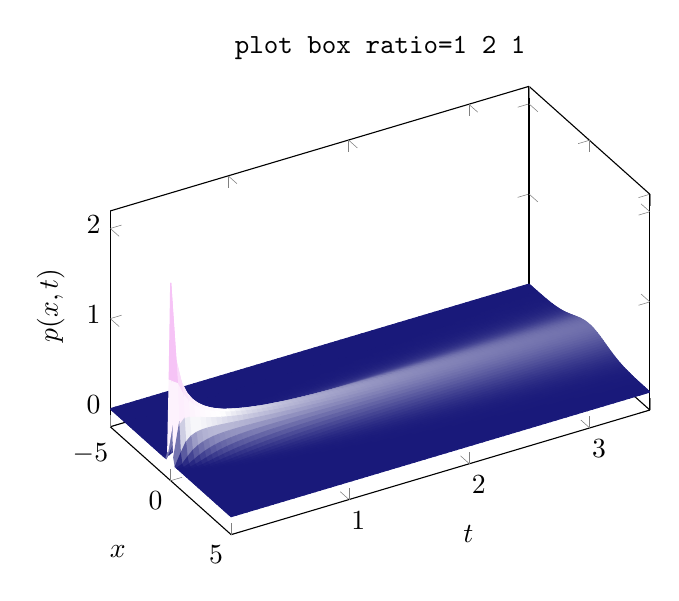
\begin{tikzpicture}
\begin{axis}[
    view/h=60,
    plot box ratio=1 2 1,
    colormap={violet}{[1cm] rgb255(0cm)=(25,25,122)
        color(1cm)=(white) rgb255(5cm)=(238,140,238)},
    xlabel=$x$,
    ylabel=$t$,
    zlabel={$p(x,t)$},
    shader=flat,
    title=\texttt{plot box ratio=1 2 1},
]
    \addplot3 [surf,y domain=0.02:3.5,samples=81]
        {1/(2*sqrt(pi*y)) * exp(0-x^2/y)};
    % the '0' is a workaround for a bug in PGF 2.00
\end{axis}
\end{tikzpicture}
\end{codeexample}

    此键仅适用于三维坐标轴。缩放之后，坐标轴会被拉伸以填充此图的 |width| 和 |height|。因此，对于特定视图，|plot box ratio| 的效果可能会被这种拉伸所抵消。
\end{pgfplotskey}

\begin{pgfplotskey}{3d box=\mchoice{background,complete,complete*} (initially background)}
\label{pgfplots:key:3dbox}
    允许配置带盒三维坐标轴的外观。

    只输入 |3d box|（不带值）即可作为 |3d box=complete| 的别名。

    选项 \declaretext{background} 是初始设置，它不绘制位于前景的坐标轴线（和网格线）。
    %
\begin{codeexample}[]
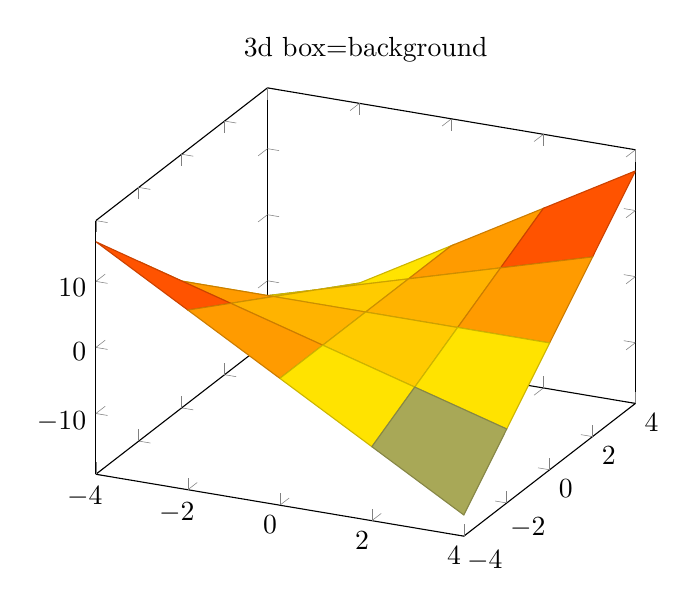
\begin{tikzpicture}
\begin{axis}[
    3d box=background,
    % pretty printing, but irrelevant:
    title={3d box=background},
    samples=5,
    domain=-4:4,
    xtick=data,
    ytick=data,
]
    \addplot3 [surf] {x*y};
\end{axis}
\end{tikzpicture}
\end{codeexample}

    选项 \declaretext{complete} 还会在前景绘制坐标轴线和刻度线，但不在前景绘制网格线。其结果是得到一个完整的盒：
    %
\begin{codeexample}[]
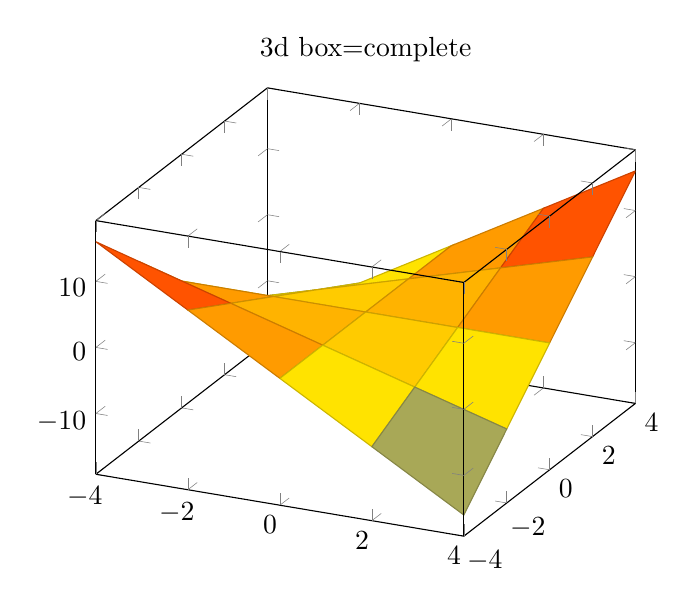
\begin{tikzpicture}
\begin{axis}[
    3d box,% same as 3d box=complete
    % pretty printing, but irrelevant:
    title={3d box=complete},
    samples=5,
    domain=-4:4,
    xtick=data,
    ytick=data,
]
    \addplot3 [surf] {x*y};
\end{axis}
\end{tikzpicture}
\end{codeexample}

    最后，选项 \declaretext{complete*} 与 |complete| 相同，但它还会在前景绘制网格线。
    %
\begin{codeexample}[]
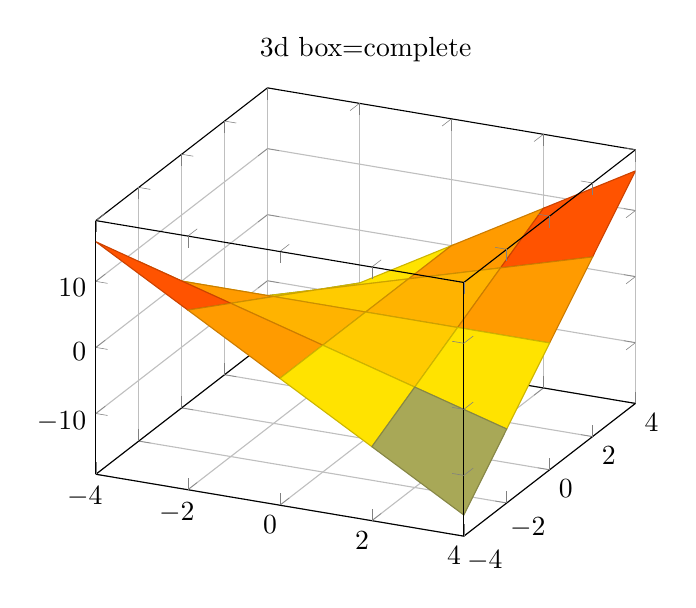
\begin{tikzpicture}
    \begin{axis}[
        3d box=complete,
        grid=major,
        title={3d box=complete},
        samples=5, domain=-4:4,
        xtick=data, ytick=data,
    ]
        \addplot3 [surf] {x*y};
    \end{axis}
\end{tikzpicture}%
~
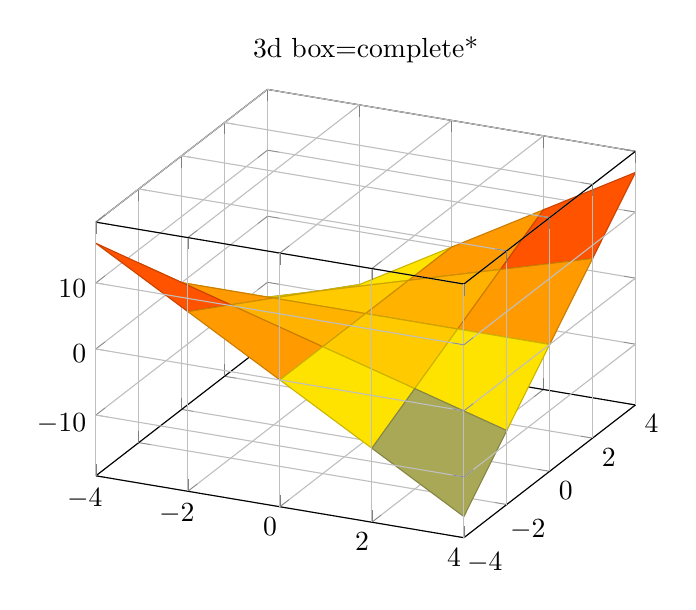
\begin{tikzpicture}
    \begin{axis}[
        3d box=complete*,
        grid=major,
        title={3d box=complete*},
        samples=5, domain=-4:4,
        xtick=data, ytick=data,
    ]
        \addplot3 [surf] {x*y};
    \end{axis}
\end{tikzpicture}
\end{codeexample}

    在任何前景部分被实际处理\emph{之前}，会安装样式 |every 3d box foreground|。这允许你将前景坐标轴组件（例如 |tick style| 或 |axis line style|）的外观与背景组件分开修改。

    请注意，|3d box=complete| \emph{仅} 适用于带盒坐标轴，也就是说要与 |axis lines=box| 一起使用。使用其他组合是错误的。
\end{pgfplotskey}


\subsection{坐标轴线变体}
\label{sec:pgfplots:axislines:3d}

三维坐标轴同样受益于 Section~\ref{sec:pgfplots:axislines} 中讨论的 |axis lines=box| 或 |axis lines=center| 样式。选项 |axis lines=box| 是标准方式，它绘制一个盒（可能受 |3d box=complete| 键影响）。选项 |axis lines=center| 将三条坐标轴都画成穿过原点。由于没有深度信息，可能需要将此键与 |axis on top| 结合使用。

\begin{codeexample}[]
% Attention: use compat=1.8 or higher
% to repair label positions
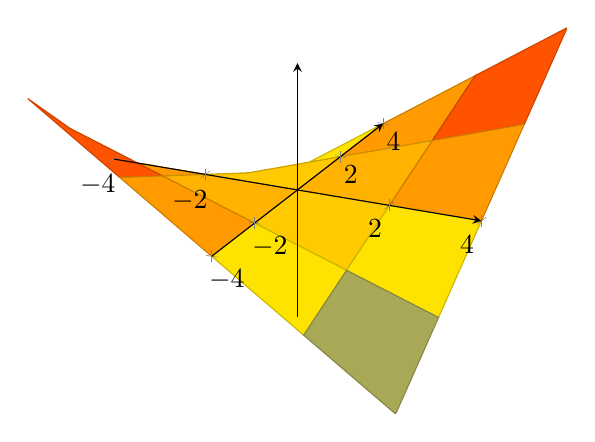
\begin{tikzpicture}
\begin{axis}[
    axis lines=center,
    axis on top,
    samples=5, domain=-4:4,
    xtick=data, ytick=data,
    ztick=\empty, % no z ticks here
]
    \addplot3 [surf] {x*y};
\end{axis}
\end{tikzpicture}
\end{codeexample}

其余选项 |axis lines*=left| 和 |axis lines*=right| 会选择不同的坐标轴集合，使得刻度标签和坐标轴标签不会干扰绘图内容。`|*|' 会抑制那些主要适用于二维坐标轴的特殊样式的使用，参见 |axis lines| 的文档。这样一组坐标轴始终位于二维投影的边界上。

选项 |axis lines*=left| 选择位于左侧（或下方，视情况而定）的一组坐标轴，而选项 |axis lines*=right| 选择位于右侧（或上方，视情况而定）的一组坐标轴：

\begin{codeexample}[]
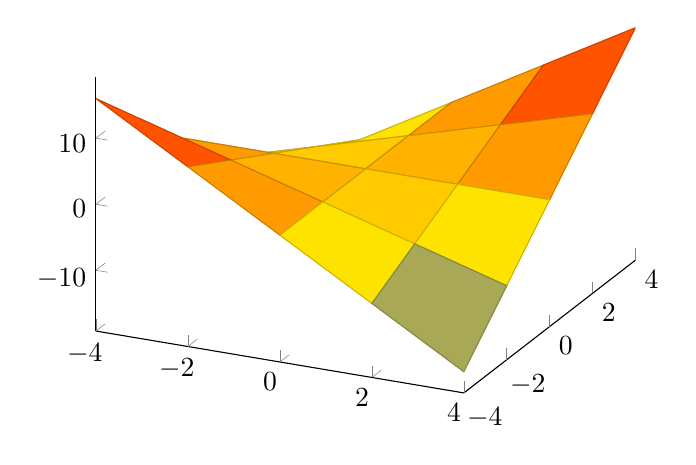
\begin{tikzpicture}
\begin{axis}[
    axis lines*=left,
    samples=5, domain=-4:4,
    xtick=data, ytick=data,
]
    \addplot3 [surf] {x*y};
\end{axis}
\end{tikzpicture}
\end{codeexample}

\begin{codeexample}[]
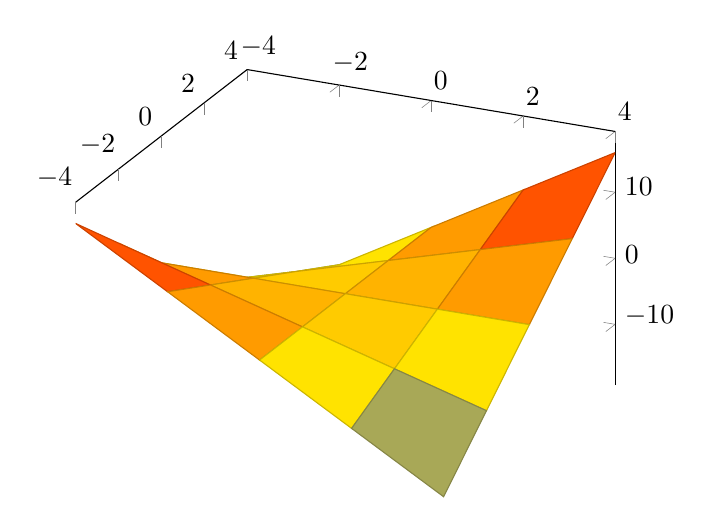
\begin{tikzpicture}
\begin{axis}[
    axis lines*=right,
    samples=5, domain=-4:4,
    xtick=data, ytick=data,
]
    \addplot3 [surf] {x*y};
\end{axis}
\end{tikzpicture}
\end{codeexample}

不能混用不同的样式，例如 |axis x line=center,axis z line=top|。

}
